\documentclass[compress, 8pt]{beamer}
% \documentclass[handout, 8pt]{beamer}
\usepackage[utf8]{inputenc}

% Notes to self: \nts[color option]{text that is a note}
\newif\ifshowcomments
% \showcommentstrue % uncomment to show


% Standard packages
\usepackage{hyperref} % Include links
\usepackage{setspace} % More control over local line spacing: http://felix11h.github.io/blog/line-spacing-beamer
% Math
\usepackage{amsthm, amsmath, mathtools}
\usepackage{appendixnumberbeamer}
% Multi=row and column
\usepackage{multirow,multicol}
% multiline columns
\usepackage{tabularx}


\usepackage{ifthen}

\usepackage{amsbsy}

%%%%%%%%%%%%%%
% Formatting %
%%%%%%%%%%%%%%

% Outer theme
\useoutertheme[subsection=false]{miniframes}
% Fix to display navigational dots; dots only shown for subsections
% Can comment out to have no dots in presentation
\AtBeginSection[]{\subsection{}}
% Font
\usepackage[default]{cantarell}

% Colors
\usepackage{xcolor}
% UCSD color palette: http://ucpa.ucsd.edu/brand/elements/color-palette/
\definecolor{DarkBlue}{RGB}{24, 43, 73}
\definecolor{MainBlue}{RGB}{0, 106, 150}
\definecolor{LightBlue}{RGB}{0, 198, 215}
\definecolor{Green}{RGB}{110 150 59}
\definecolor{Yellow}{RGB}{255 205 0}
\definecolor{LightYellow}{RGB}{243 29 0}
\definecolor{Gold}{RGB}{198 146 20}
\definecolor{Orange}{RGB}{252 137 0}
\definecolor{LightGrey}{RGB}{182, 177, 169}
\definecolor{DarkGray}{RGB}{116 118 120}
\definecolor{DarkPurple}{RGB}{25 0 51}
\definecolor{Purple}{RGB}{55 24 81}
\definecolor{Maroon}{HTML}{6A123D}
\definecolor{HunterPurple}{HTML}{5F259F}
\definecolor{HunterGold}{HTML}{FFC72A}
\definecolor{HunterGray}{HTML}{EEECF0}


% Hyperlink colors
\hypersetup{
  colorlinks   = true, %Colours links instead of ugly boxes
  urlcolor     = Maroon, %Colour for external hyperlinks
  linkcolor    = DarkGray, %Colour of internal links
  citecolor   = HunterPurple %Colour of citations
}


% Learned using: https://ramblingacademic.com/2015/12/how-to-quickly-overhaul-beamer-colors/
% To change additional sections: http://www.cpt.univ-mrs.fr/~masson/latex/Beamer-appearance-cheat-sheet.pdf
\setbeamercolor{palette primary}{bg=HunterPurple,fg=white}
\setbeamercolor{palette secondary}{bg=HunterPurple,fg=white}
\setbeamercolor{palette tertiary}{bg=HunterPurple,fg=white}
\setbeamercolor{palette quaternary}{bg=HunterPurple,fg=white}
\setbeamercolor{structure}{fg=HunterPurple} % itemize, enumerate, etc
\setbeamercolor{section in toc}{fg=HunterPurple} % TOC sections
\setbeamercolor{section in head/foot}{bg=HunterPurple,fg=LightGrey}
%\setbeamercolor{navigation symbols}{bg=Gold, fg=Gold}
\setbeamercolor{alerted text}{fg=MainBlue}
\beamertemplatenavigationsymbolsempty
%tem
%\setbeamertemplate{itemize items}

% Make bullet size smaller
\setbeamertemplate{itemize item}{\tiny\raise1.4pt\hbox{$\blacktriangleright$}}
\setbeamertemplate{itemize subitem}{--}
% make bullet closer to the text
\setlength{\labelsep}{.8ex}

% get rid of 'Figure: ' in caption
\setbeamertemplate{caption}{\raggedright\insertcaption\par}
% Caption flushed left
\usepackage{caption}
\captionsetup{%
    labelformat=empty,
    font=small,
    singlelinecheck=false,
    tableposition=top
}


%%%%%%%%%%%%%%%%
% New commands %
%%%%%%%%%%%%%%%%

\ifshowcomments
\newcommand{\nts}[2][DarkGray]{\setbeamercolor{taras comment}{fg=#1}{\usebeamercolor[fg]{taras comment}\setbeamercolor{item}{fg = taras comment.fg}\emph{#2}}}
\else 
\newcommand{\nts}[2][DarkGray]{}
\fi

% Timed color highlights
\newcommand<>{\blue}[1]{\textbf{\color#2{MainBlue}#1}}
\newcommand<>{\mblue}[1]{{\color#2{MainBlue}#1}}
\newcommand<>{\green}[1]{\textbf{\color#2{Green}#1}}
\newcommand<>{\mgreen}[1]{{\color#2{Green}#1}}

\newcommand{\EE}{\mathbf{E}}
\newcommand{\PP}{\mathbf{P}}
\newcommand{\llog}[1]{\log \left( #1 \right)}
\newcommand{\Cov}[1]{\text{Cov} \left( #1 \right)}
\newcommand{\Var}[1]{\text{Var} \left( #1 \right)}
\newcommand{\XX}{\mathbf{X}}
\newcommand{\xx}{\mathbf{x}}

\newcommand{\br}[1]{\left\{ #1 \right\}}
\newcommand{\sbr}[1]{\left[ #1 \right]}
\newcommand{\pr}[1]{\left( #1 \right)}
\newcommand{\ce}[2]{\left[\left. #1 \right\vert #2 \right]}
\newcommand{\cls}[2]{\left. #1 \right\vert #2}
\newcommand{\crs}[2]{#1 \left\vert #2 \right.}
\newcommand{\ceil}[1]{\left\lceil #1 \right\rceil}

% Beamer buttons
% bottom buttom: \bbutton{name_of_link}{Text to print}
\newcommand{\bbutton}[2]{
    \begin{tikzpicture}[remember picture, overlay]
    \node[shift={(-1.4cm,0.5cm)}]() at (current page.south east){%
    \hyperlink{#1}{\beamergotobutton{#2}}};    
    \end{tikzpicture}
}    
% here button
\newcommand{\hbutton}[2]{
    \hyperlink{#1}{\beamergotobutton{#2}}
}
% Cite command: cc
\newcommand{\nn}[2][DarkGray]{{\small \color{#1} #2}}
\newcommand{\ccdoi}[2]{\href{https://doi.org/#1}{\nn{#2}}}
\newcommand{\ccurl}[2]{\href{#1}{\nn{#2}}}

% change slide width on a single slide
% source: https://tex.stackexchange.com/questions/160825/modifying-margins-for-one-slide/242073
\newcommand\Wider[2][3em]{%
\makebox[\linewidth][c]{%
  \begin{minipage}{\dimexpr\textwidth+#1\relax}
  \raggedright#2
  \end{minipage}%
  }%
}

% To remove sections from appendix
% source: https://tex.stackexchange.com/questions/37127/how-to-remove-some-pages-from-the-navigation-bullets-in-beamer
\makeatletter
\let\beamer@writeslidentry@miniframeson=\beamer@writeslidentry
\def\beamer@writeslidentry@miniframesoff{%
  \expandafter\beamer@ifempty\expandafter{\beamer@framestartpage}{}% does not happen normally
  {%else
    % removed \addtocontents commands
    \clearpage\beamer@notesactions%
  }
}
\newcommand*{\miniframeson}{\let\beamer@writeslidentry=\beamer@writeslidentry@miniframeson}
\newcommand*{\miniframesoff}{\let\beamer@writeslidentry=\beamer@writeslidentry@miniframesoff}
\makeatother

%%%%%%%%%%%%%%%%%%%%
% Figures and tikz %
%%%%%%%%%%%%%%%%%%%%

% \usepackage{pgfplots} % maybe for tikz axes?
\usepackage{graphicx} % Include figures
\usepackage{tikz} % Draw figures with tikz
\usetikzlibrary{positioning} % to use right=of <node> syntax
\usetikzlibrary{shapes} % for other node shapes; see http://www.texample.net/tikz/examples/node-shapes/
% \usetikzlibrary{shapes.multipart} % multiline nodes in tikz
% \usetikzlibrary{shapes.arrows} % arrow nodes in tikz
% \usetikzlibrary{shapes.misc} % miscellaneous nodes in tikz; for rounded rectangles
% \usetikzlibrary{shapes.geometric} % geometric nodes in tikz; fortriangles
% \usetikzlibrary{shapes.ellipse} % geometric nodes in tikz; fortriangles

% Presentation specific tikz
%\usetikzlibrary{tikzmark} % to use tikzmarkto add braces to itemize
% \usetikzlibrary{calc} % for widthof
% \tikzset{
%     above label/.style={
%         above = 5pt,
%         %font=\footnotesize,
%         text height = 1.5ex,
%         text depth = 1ex,
%     },
%     below label/.style={  
%         below=4pt,
%         %font=\footnotesize,
%         text height = 1.5ex,
%         text depth = 1ex
%     },
%     brace label/.style={
%         below = 4pt,
%         font=\footnotesize,
%         text height = 1.5ex,
%         text depth = 1ex
%     },
%     brace/.style={
%         decoration={brace, mirror},
%         decorate
%     }
% }

% For every picture that defines or uses external nodes, you'll have to
% apply the 'remember picture' style. To avoid some typing, we'll apply
% the style to all pictures.
%\tikzstyle{every picture}+=[remember picture]

% To avoid a warning
% \pgfplotsset{compat=1.7}
\usepackage[normalem]{ulem}

%%%%%%%%%%%%%%%%%%%%%%%%%%%%%%%%%%%%%%%%%%%%%%%%%%%%%%%%%%%%%%%%%%%%%%%%%%%%%%
% Paths to figures
\usepackage{subcaption}

% Avoid a warning on mac; can introduce a warning (and maybe a break) on windows
% \usepackage{etex}
% Avoid a warning
\let\Tiny=\tiny

%Information to be included in the title page:
\title{Linear regression}
\subtitle{ECON726}
\author[]{Tara Sullivan}
\institute{
Tara Sullivan \\
\textit{tara.sullivan55@login.cuny.edu}
}
\date{
\today
\nts{\\
\medskip
Notes/comments are in gray and will be excluded from the presentation.
}
}

% plot graphs with pgfplots
\usepackage{pgfplots}
\pgfplotsset{compat=newest}
\usepgfplotslibrary{groupplots}
\usepgfplotslibrary{dateplot}
\pgfplotsset{compat=newest,
    every axis/.style={
        axis y line*=left,
        axis x line*=bottom,
        % allows for multi-line legend entries
        legend style={cells={align=left}},
        % allows for multi-line titles
        title style={align=center},
    },
}

% For animations using underbrace 
% Source: https://tex.stackexchange.com/a/565866
\usepackage{xparse, letltxmacro}
\LetLtxMacro{\oldunderbrace}{\underbrace}
\DeclareDocumentCommand{\underbrace}{d<> m e{_}}{%
  \IfValueTF{#1}{% IF <overlay-specification> given
    % using global onlside flag, cf. p82 beamer manual v3.59
    \oldunderbrace{#2\onslide<#1>}_{#3}\onslide%
  }{% ELSE
    \oldunderbrace{#2}_{#3}
  }%
}%

\usetikzlibrary{decorations.pathreplacing,calligraphy}

%%%%%%%%%%%%%%%%%%%%%%%%%%%%%%%%%%%%%%%%%%%%%%%%%%%%%%%%%%%%%%%%%%%%%%%%%%%%%%%%
\begin{document}    
%\beamertemplatenavigationsymbolsempty


%%%%%%%%%%%%%%%%%%%%%%%%%%%%%%%%%%%%%%%%%%%%%%%%%%%%%%%%%%%%%%%%%%%%%%%%%%%%%%%%
\begin{frame}
\titlepage
% \tikzset{external/figure name={intro_}}
\end{frame}

%%%%%%%%%%%%%%%%%%%%%%%%%%%%%%%%%%%%%%%%%%%%%%%%%%%%%%%%%%%%%%%%%%%%%%%%%%%%%%%%
\begin{frame}{Housekeeping}

\textbf{Last week's homework:}
\begin{itemize}
    \item I will try to provide comments on your paper ideas
    \item Please email me or set up office hours if you would like to discuss
\end{itemize}

\vspace{3ex}
\textbf{Homework}
\begin{itemize}
    \item Read MHE 3.3.1
    \begin{itemize}
        \item Review 3.1. and 3.2., if you're still shaky on the concepts
    \end{itemize}
\end{itemize}

\vspace{3ex}
\textbf{Today:}
\begin{itemize}
    \item Reviewing regression from Mostly Harmless Econometrics
    \item Also reviewing regression from \href{https://causalml-book.org}{Causal ML book}
    \begin{itemize}
        \item Chapter 1: Predictive Inference with Linear Regression in Moderately High Dimensions
    \end{itemize}
\end{itemize}

\end{frame}

%%%%%%%%%%%%%%%%%%%%%%%%%%%%%%%%%%%%%%%%%%%%%%%%%%%%%%%%%%%%%%%%%%%%%%%%%%%%%%%%
\begin{frame}{Empirical project}

\textbf{Paper selection}: Due \textbf{September 28} [5\% of final grade]
\begin{itemize}
    \item Done!
\end{itemize}

\textbf{Project plan}: Due \textbf{October 12} [15\% of final grade] 
\begin{itemize}
\item This paper should be your first effort at addressing points (1) and (2) above.
Summarize the public policy or business context of the paper. Write down the
specific question the paper is evaluating. Discuss the data your are using (both your replication data, and data for your extension). Verify that you can access the data and replication package. Discuss the extensions you are considering, and, if necessary, where you will be getting that data. Verify that you’ve read the paper.
\end{itemize} 

\textbf{Replication results}: Due \textbf{November 2}: [10\% of final grade]
\begin{itemize}
\item You should submit some of your main replication results. The final results should be formatted as tables and charts in a word document or PDF, submitted on Brightspace. Your code and data should accessible on GitHub.
\end{itemize}

\textbf{Presentation}: Due \textbf{December 1} \& \textbf{December 8} [10\% of final grade]
\begin{itemize}
\item Prepare a 10 minute presentation on your paper. Focus on the research question, main result, and one extension. 
\end{itemize}

\textbf{Final Paper}: Due \textbf{December 11} [40\% of final grade]
\begin{itemize}
\item Your paper should contain 6-10 pages of text, and 3-6 pages of figures (double spaced, 12 point font).
You must provide the code and data to replicate your findings. 
Your final project should be submitted on Brightspace, and your code and data should be uploaded to github (note: if your data is too large to upload to github, let me know). 
\end{itemize}

\end{frame}


% %%%%%%%%%%%%%%%%%%%%%%%%%%%%%%%%%%%%%%%%%%%%%%%%%%%%%%%%%%%%%%%%%%%%%%%%%%%%%%%%
% \begin{frame}{Initial paper selection: brightspace assignment}

% Submit one paper you are considering for your replication project (it can be the paper from the previous assignment). Briefly describe the causal effect of interest and methodology, and what you may do for your extension. For all papers, please submit:

% A link to the (published) version of the paper
% A link to the replication code or data
% What is the causal question of interest in this paper?
% What is the main method used to study this causal question?

% Notes:

% This is your initial selection of a paper. Submitting this assignment on time will be worth 5\% of your final grade.&nbsp;
% You will be able to change your paper selection later. The goal is to answer the questions above.
% Extension notes: You will not be held to your extension choice. But start thinking about what you may do. Perhaps a robustness check of the assumptions. Or perhaps you will try to repeat this methodology in a different context, using similar or modified. Maybe you'll want to add in new control variables, and see if that changes the results. Just start thinking creatively about how you can modify the results of a paper (look at the conclusion for hints of what can be done!)

% \end{frame}



%%%%%%%%%%%%%%%%%%%%%%%%%%%%%%%%%%%%%%%%%%%%%%%%%%%%%%%%%%%%%%%%%%%%%%%%%%%%%%%
\miniframesoff
\begin{frame}{Outline}
    \tableofcontents
\end{frame}
\miniframeson



%%%%%%%%%%%%%%%%%%%%%%%%%%%%%%%%%%%%%%%%%%%%%%%%%%%%%%%%%%%%%%%%%%%%%%%%%%%%%%%%
\section[CEF]{Conditional Expectations Function}
\miniframesoff
\begin{frame}
    \tableofcontents[currentsection]
\end{frame}
\miniframeson
%%%%%%%%%%%%%%%%%%%%%%%%%%%%%%%%%%%%%%%%%%%%%%%%%%%%%%%%%%%%%%%%%%%%%%%%%%%%%%%

%%%%%%%%%%%%%%%%%%%%%%%%%%%%%%%%%%%%%%%%%%%%%%%%%%%%%%%%%%%%%%%%%%%%%%%%%%%%%%%%
\begin{frame}{CEF theorems}

Law of iterated expectations:
\begin{equation*}
    \EE [Y ] = \EE \left[ \EE[Y \vert X] \right]
\end{equation*}

CEF decomposition property: \begin{align*}
    Y_i &= \EE[Y_i \vert X_i] + \epsilon_i,
\end{align*}
CEF prediction property:
\begin{align*}
\EE[Y_i \vert X_i] = \arg \min_{m(X_i)} \EE \left[(Y_i - m(X_i))^2\right]
\end{align*}
ANOVA theorem:
\begin{equation*}
    \Var{Y_i} = \Var{\EE[Y_i \vert X_i]} + \EE \left[ \Var{Y_i \vert X_i} \right]
\end{equation*}

\end{frame}

%%%%%%%%%%%%%%%%%%%%%%%%%%%%%%%%%%%%%%%%%%%%%%%%%%%%%%%%%%%%%%%%%%%%%%%%%%%%%%%%
\begin{frame}{CEF Theorems}


Why are these theorems helpful?
\begin{itemize}
    \item Decompositions are helpful for summarizing data
    \item Work in populations as well as samples
    \item Do not rely on the linearity of CEF assumptions
\end{itemize}

\end{frame}





%%%%%%%%%%%%%%%%%%%%%%%%%%%%%%%%%%%%%%%%%%%%%%%%%%%%%%%%%%%%%%%%%%%%%%%%%%%%%%%%
\section[Regression]{Regression}
\miniframesoff
\begin{frame}
    \tableofcontents[currentsection]
\end{frame}
\miniframeson
%%%%%%%%%%%%%%%%%%%%%%%%%%%%%%%%%%%%%%%%%%%%%%%%%%%%%%%%%%%%%%%%%%%%%%%%%%%%%%%%


%%%%%%%%%%%%%%%%%%%%%%%%%%%%%%%%%%%%%%%%%%%%%%%%%%%%%%%%%%%%%%%%%%%%%%%%%%%%%%%%
\begin{frame}{Regression}

    Regression analysis is a \alert<2->{\textbf{statistical method}} for estimating the relationship between:
    \begin{itemize}
        \item Dependent variable
        \begin{itemize}
            \item $Y$, outcome variable, response variable, label
        \end{itemize}
        \item One or more independent variables 
        \begin{itemize}
            \item $X$, $(X_1, \dots, X_p)^\prime$, regressors, predictors, covariates, explanatory variables, features
        \end{itemize}
    \end{itemize}

    % 2 on
    \vspace{2ex}
    \pause
    Why do we clarify that this is a \alert<2->{\textbf{statistical method}}?
    \begin{itemize}
        \item Right now, we're saying \textbf{nothing} about causality
        \item Regression is a statistical tool that summarizes a relationship between variables
        \item Linking regression to causality takes further assumptions 
    \end{itemize}

    \vspace{2ex}
    Regression is important far beyond causal analysis
    \begin{itemize}
        \item Key in prediction and forecasting
        \item Heavily overlaps with machine learning
    \end{itemize}

\end{frame}

% %%%%%%%%%%%%%%%%%%%%%%%%%%%%%%%%%%%%%%%%%%%%%%%%%%%%%%%%%%%%%%%%%%%%%%%%%%%%%%%%
% \begin{frame}{}

% The \textbf{regression function} is the best-fitting line generated by minimizing expected squared errors.
% \begin{itemize}
%     \item ``Regression'' on its own doesn't say anything about causality
%     \item Today, we are just considering the population regression coefficients, derived from the population least squares problem. 
% \end{itemize}

% \vspace{3ex}
% Regression is closely tied to the conditional expectations function (CEF)
% \begin{itemize}
%     \item In MHE, the authors discuss how the link between the CEF and regression function can be explained in three ways
% \end{itemize}

% \end{frame}


%%%%%%%%%%%%%%%%%%%%%%%%%%%%%%%%%%%%%%%%%%%%%%%%%%%%%%%%%%%%%%%%%%%%%%%%%%%%%%%%
\begin{frame}{Regression model}
{
    \small
\begin{columns}
\begin{column}{0.5\textwidth}
\begin{itemize}
    \item $Y_i$: dependent variable
    \item $\XX_i$: $p \times 1$ vector of covariates
    \begin{itemize}
        \item Elements $X_{pi}$
        \item Often assume $X_{1i} = 1$
        \item Often drop the $i$ subscript
    \end{itemize}
    \item Unknown scalar or vector $\beta$
    \item Unobservable error terms $\epsilon_i$
\end{itemize}
\end{column}
\begin{column}{0.2\textwidth}
\begin{align*}
\XX_i &= \begin{bmatrix} X_{1i} \\ \vdots \\ X_{pi} \end{bmatrix} \\
&= \begin{bmatrix}
    X_{1i}, X_{2i}, \dots, X_{pi}
\end{bmatrix}^\prime
\end{align*}
\end{column}
\end{columns}
}

Most regression models propose that $Y_i$ is a function of $\XX_i$, $\beta$, and $\epsilon_i$:
\begin{equation*}
    Y_i = f(\XX_i, \beta) + \epsilon_i
\end{equation*}
\textbf{Goal:} is to estimate the function $f(\XX_i, \beta)$ that most closely fits the data. 

\pause
\vspace{2ex}
To start, we will consider \textbf{linear regression} in the \textbf{population}. 
\begin{itemize}
    \item Linear regression function means $f(\XX_i, \beta)$ is a linear function 
    \item Why population?
    \begin{itemize}
    \item Unlimited amounts of data to compute population \textbf{moments} ($\EE[Y]$, $\EE[\XX_i]$, $\EE [YX]$, $\EE [XX^\prime]$)
    \item Define ideal quantities in the population
    \item Then return to estimating these quantities using sample of observations drawn from the population
    \end{itemize}

\end{itemize}


\end{frame}


%%%%%%%%%%%%%%%%%%%%%%%%%%%%%%%%%%%%%%%%%%%%%%%%%%%%%%%%%%%%%%%%%%%%%%%%%%%%%%%%
\begin{frame}{Best linear prediction rule (in the population)}
    First goal: construct the best linear predictor for $Y$ using $\XX$ (dropping $i$ subscript):
    \begin{equation*}
        \sum_{j=1}^p \beta_j X_j = \beta^\prime \XX, \quad\text{for } \ \beta = \begin{bmatrix}
        \beta_1, \dots, \beta_p
        \end{bmatrix}^\prime
    \end{equation*}
    $\beta$ are the \textbf{regression parameters} or \textbf{coefficients}

    \vspace{2ex}
    Define $\beta$ as the solution to the \textbf{Best Linear Prediction (BLP) Problem}:

    \begin{equation*}
        \beta = \arg \min_{b} \underbrace{\EE \left[ \left(Y - b^\prime \XX \right)^2 \right]}_{\text{MSE}}
    \end{equation*}
\begin{itemize}
    \item Find the $b$ that minimizes the \textbf{Mean Squared Error (MSE)} using the \textbf{linear rule}:
    \begin{equation*}
        b^\prime X = \sum_{j=1}^p b_j X_j, \quad b = (b_1, \dots, b_p)^\prime
    \end{equation*}
\end{itemize}
Solution to this optimization problem is the \textbf{Best Linear Predictor} of $Y$ using $X$ 
\begin{itemize}
    \item Technically, best linear prediction rule among all linear prediction rules, according to the MSE
\end{itemize}


\end{frame}

%%%%%%%%%%%%%%%%%%%%%%%%%%%%%%%%%%%%%%%%%%%%%%%%%%%%%%%%%%%%%%%%%%%%%%%%%%%%%%%%
\begin{frame}{Matrix formation of OLS}

Suppose the relationship between $Y_i$ and $Z_i$ can be written as:
\begin{equation*}
    Y_i = \beta_0 + \beta_1 Z_i + \epsilon_i
\end{equation*}
We define our matrices $X_i$ and $\beta$ as:
\begin{equation*}
    X_i = \begin{bmatrix} 1 \\ Z_i \end{bmatrix},
    \quad\quad
    \beta = \begin{bmatrix} \beta_0 \\ \beta_1 \end{bmatrix}
\end{equation*}
We can write this in matrix form as:
\begin{align*}
    Y_i =& 1 \cdot \beta_0 + Z_i \cdot \beta_1 \\
    =& \begin{bmatrix} 1 &Z_{i} \end{bmatrix} \cdot \begin{bmatrix} \beta_0 \\ \beta_1 \end{bmatrix} + \epsilon_i \\
    =& X_i^\prime \beta + \epsilon_i
\end{align*}


\end{frame}

%%%%%%%%%%%%%%%%%%%%%%%%%%%%%%%%%%%%%%%%%%%%%%%%%%%%%%%%%%%%%%%%%%%%%%%%%%%%%%%%
\begin{frame}{Regression and CEF - Best Linear Predictor}

\textbf{MHE Thm. 3.1.5: The best linear predictor theorem}: The function $X_i^\prime \beta$ is the best \textbf{linear} predictor of $Y_i$ given $X_i$, in an MSE sense

\vspace{1ex}
\emph{Proof:} Recall the population least squares problem:
\begin{equation*}
    \beta = \arg \min_b \EE \left[ \left(Y_i - \XX_i^\prime b\right)^2 \right]
\end{equation*}
$\beta = \EE [X_i X_i^\prime]^{-1} \EE [X_i Y_i]$ solves this problem, and thus is the best \textbf{linear} predictor of $Y_i$ given $X_i$

\vspace{3ex}
Context:
\begin{itemize}
    \item Consider how the CEF, $\EE [Y_i \vert X_i]$, is the best MSE predictor of $Y_i$ given $X_i$ in the class of all functions of $X_i$
    \item The population regression is the best MSE predictor of $Y_i$ given $X_i$ in the class of \textbf{linear} functions of $X_i$
\end{itemize}
\end{frame}


%%%%%%%%%%%%%%%%%%%%%%%%%%%%%%%%%%%%%%%%%%%%%%%%%%%%%%%%%%%%%%%%%%%%%%%%%%%%%%%%
\begin{frame}{First order condition}
    Given Best Linear Prediction Problem:
    \begin{equation*}
        \arg \min_{b} \EE \left[ \left(Y_i - b^\prime \XX_i \right)^2 \right]
    \end{equation*}
    To find the $b$ that minimizes the MSE, you set the derivative equal to zero. This is called the \textbf{first order condition}. 
\begin{equation*}
    \EE [(Y_i - b^\prime \XX_i) \XX_i] = 0
\end{equation*}
This is also referred to as the \textbf{Normal Equation}.

\vspace{2ex}
To find the solution, use linear algebra:
\begin{align*}
    0 &= \EE[\XX_i (Y_i - b^\prime \XX_i)] \\
    0 &= \EE [\XX_i Y_i - \XX_i \XX_i^\prime b] \\
    0 &= \EE [\XX_i Y_i] - \EE [\XX_i \XX_i^\prime b]\\
    \EE [\XX_i \XX_i^\prime b] &= \EE [\XX_i Y_i] \\
    \EE [\XX_i \XX_i^\prime] b &= \EE [\XX_i Y_i] \\
    b &= \EE [\XX_i \XX_i^\prime]^{-1} \EE [\XX_i Y_i]
\end{align*}

\end{frame}



%%%%%%%%%%%%%%%%%%%%%%%%%%%%%%%%%%%%%%%%%%%%%%%%%%%%%%%%%%%%%%%%%%%%%%%%%%%%%%%%
\begin{frame}{Population residual}
Regression coefficient solves:
\begin{equation*}
    \beta = \arg \min_b \EE \left[ \left(Y_i - \XX_i^\prime b\right)^2 \right]
\end{equation*}
First order condition / Normal Equation:
\begin{equation*}
    \EE [\XX_i (Y_i - \XX_i^\prime b)] = 0
\end{equation*}
Solution:
\begin{equation*}
    \beta = \EE [\XX_i \XX_i^\prime]^{-1} \EE [\XX_i Y_i]
\end{equation*}
Define the \textbf{residual} or \textbf{regression error} as:
\begin{equation*}
    \epsilon_i = Y_i - \beta^\prime \XX_i
\end{equation*}
Can write the Normal equation as:
\begin{equation*}
    \EE [ \epsilon_i \XX_i ] = 0
\end{equation*}
where $\epsilon_i$ is \textbf{orthogonal} to $\XX_i$, leading to the decomposition:
\begin{equation*}
    Y_i = X_i^\prime \beta + \epsilon_i, \quad \epsilon_i \perp X_i
\end{equation*}
\begin{itemize}
    \item $X_i^\prime \beta$: part of $Y_i$ that can be (linearly) explained by $X_i$
    \item $\epsilon_i$: Unexplained/residual part of $Y_i$
\end{itemize}

% Note: by construction of the first order condtion, the population residual, $e_i$, is uncorrelated with (orthogonal to) the regressors, $X_i$:
% \begin{equation*}
%     \EE [X_i \underbrace{(Y_i - \XX_i^\prime b)}_{e_i}] = 0
% \end{equation*}
% The population residual, the part of $Y_i$ that is unexplained by the linear combination of $\XX_i$, is, by definition, uncorrelated with $\XX_i$

\end{frame}



% %%%%%%%%%%%%%%%%%%%%%%%%%%%%%%%%%%%%%%%%%%%%%%%%%%%%%%%%%%%%%%%%%%%%%%%%%%%%%%%%
% \begin{frame}{Deriving OLS coefficients}

% First order condtion 
% \begin{align*}
%     b =& \EE [X_i X_i^\prime]^{-1} \EE [X_i Y_i] \\
%     =& \EE \left[
%         \begin{matrix} 1 \\ Z_{i} \end{matrix}
%         \begin{matrix} 1 & Z_i \end{matrix}
%     \right]
%     \EE \left[
%         \begin{matrix} 1 \\ Z_i \end{matrix}
%         \begin{matrix} Y_i \end{matrix}
%     \right] \\
%     =& \EE \left[
%         \begin{matrix} 1 & Z_i \\ Z_i & Z_i^2 \end{matrix}
%     \right]
%     \EE \left[
%         \begin{matrix} Y_i \\ Z_i \cdot Y_i \end{matrix}
%     \right] \\
% \end{align*} 


% \end{frame}



%%%%%%%%%%%%%%%%%%%%%%%%%%%%%%%%%%%%%%%%%%%%%%%%%%%%%%%%%%%%%%%%%%%%%%%%%%%%%%%%
\begin{frame}{Regression and CEF - Regression CEF Theorem}

\textbf{Thm. 3.1.6: The regression CEF theorem}: The function $X_i^\prime \beta$ is the \textbf{Best \alert{Linear} Approximation} of $\EE [Y_i \vert \XX_i]$ in an MSE sense. In math:
\begin{equation}\label{eq1}
    \beta = \arg \min_b \EE \left[ \left(\EE[Y_i \vert \XX_i] - \XX_i^\prime b\right)^2 \right]
\end{equation}

\vspace{1ex}
\emph{Proof: } We know $\beta$ solves the population least squares problem:
\begin{equation}\label{eq2}
    \beta = \arg \min_b \EE \left[ \left(Y_i - \XX_i^\prime b\right)^2 \right]
\end{equation}

Applying the law of iterated expectation to the normal equation from (\ref{eq2}):
% \begin{align*}
%     \EE \left[ \XX_i (Y_i - \XX_i^\prime b) \right] =& 0 \\
%     \EE \Big[ \EE \left[ \XX_i (Y_i - \XX_i^\prime b) \right] \Big\vert \XX_i \Big] =& 0 \\
%     \EE \Big[ \XX_i \left( \EE[Y_i \vert \XX_i ] - \XX_i^\prime b  \right) \Big] =& 0
% \end{align*}
\begin{align*}
    0 =& \EE \left[ \XX_i (Y_i - \XX_i^\prime b) \right] \\
    =& \EE \Big[ \EE \left[ \XX_i (Y_i - \XX_i^\prime b) \big\vert \XX_i \right] \Big] \\
    =& \EE \Big[ \XX_i \left( \EE[Y_i \vert \XX_i ] - \XX_i^\prime b  \right) \Big]
\end{align*}
\begin{itemize}
    \item [$\implies$] First order equation (normal equation) for minimizing (\ref{eq1})
    \item [$\implies$] Best Linear Predictor of $Y_i$ is also the Best Linear Predictor for the conditional expectation of $Y_i$ given $\XX_i$
\end{itemize}


% Write:
% \begin{align*}
%      \left(Y_i - \XX_i b\right)^2 
%      &= %\left(
%          % \left(
%              \left(Y_i {\color<1>{red} -\EE [Y_i \vert X_i] + \EE [Y_i \vert X_i]} - \XX_i^\prime b\right)^2 
%          % \right)
%      %\right) 
%      \\
%      \onslide<2->{
%      &= \left(
%          \left(
%          Y_i -\EE [Y_i \vert X_i]\right) + \left(\EE [Y_i \vert X_i] - \XX_i^\prime b\right)
%      \right)^2} \\
%      \onslide<3->{
%      &= 
%          {\color<4>{red} \left(Y_i -\EE [Y_i \vert X_i]\right)^2}
%          + \left(\EE [Y_i \vert X_i] - \XX_i^\prime b\right)^2 
%          - {\color<5>{red} 2 \left(Y_i -\EE [Y_i \vert X_i]\right) \left(\EE [Y_i \vert X_i] - \XX_i^\prime b\right)}
%          }      
%  \end{align*} 
%  \begin{itemize}
%      \onslide<4->{\item First term doesn't involve $b$}
%      \onslide<5->{\item Last term is zero by CEF decomposition property}
%  \end{itemize}
% \onslide<6->{$\implies$ CEF approximation is the same as the least squares approximation}
\end{frame}

%%%%%%%%%%%%%%%%%%%%%%%%%%%%%%%%%%%%%%%%%%%%%%%%%%%%%%%%%%%%%%%%%%%%%%%%%%%%%%%%
\begin{frame}{Regression and CEF}

Link between CEF and regression:
\begin{itemize}
    \item Regression provides the best \textbf{linear} predictor for the dependent variable $Y_i$ in the same way the CEF is the best unrestricted predictor of the dependent variable

    \item If we're trying to predict $\EE[Y_i \vert X_i]$ (not $Y_i$), then regression provides the best linear approximation (even if $\EE [Y_i \vert X_i]$ is nonlinear)
\end{itemize}


\end{frame}


%%%%%%%%%%%%%%%%%%%%%%%%%%%%%%%%%%%%%%%%%%%%%%%%%%%%%%%%%%%%%%%%%%%%%%%%%%%%%%%%
\begin{frame}{CEF of log weekly wages}

\begin{figure}
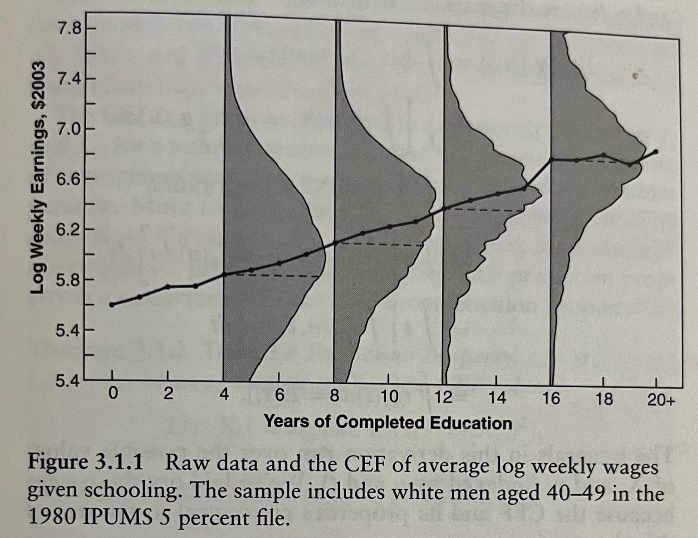
\includegraphics[scale=0.8]{img/CEF-example.png}
\end{figure}

\end{frame}

%%%%%%%%%%%%%%%%%%%%%%%%%%%%%%%%%%%%%%%%%%%%%%%%%%%%%%%%%%%%%%%%%%%%%%%%%%%%%%%%
\begin{frame}{Linear approximation of CEF}

\begin{figure}
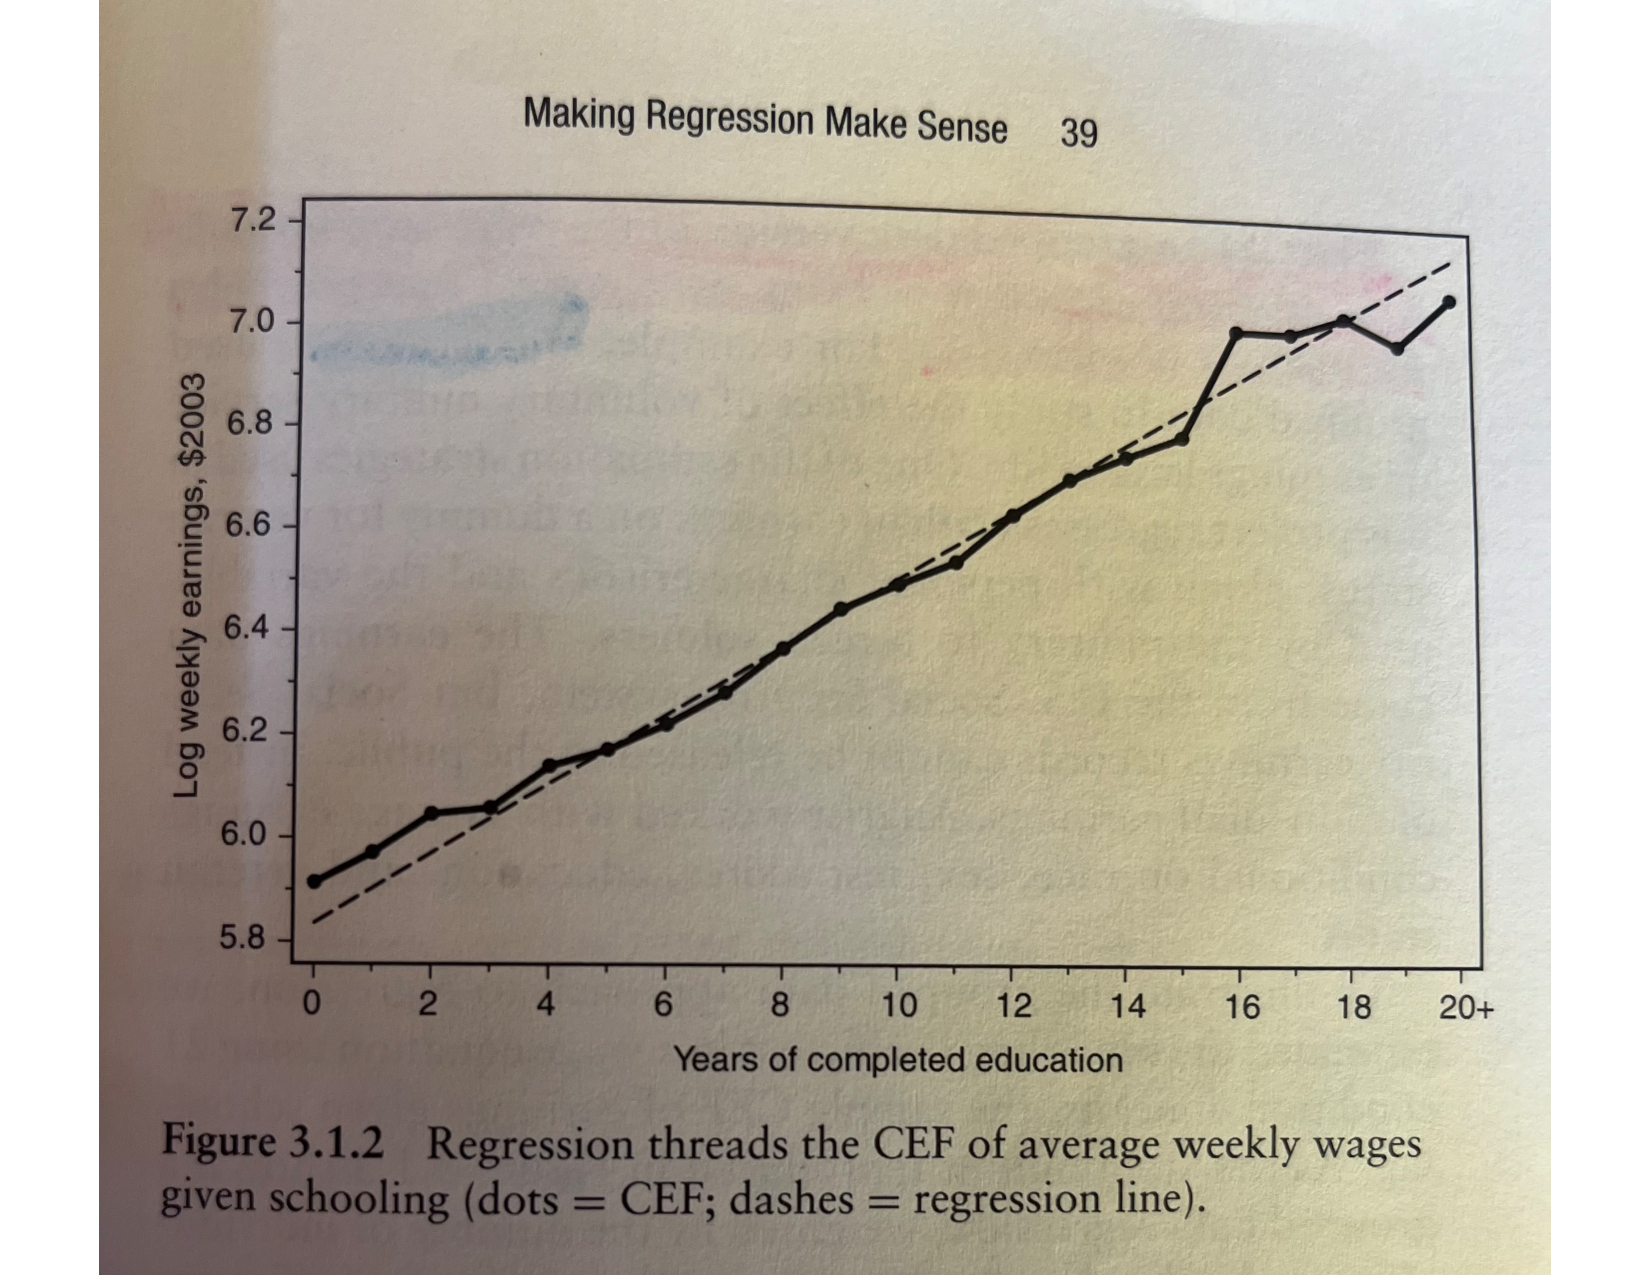
\includegraphics[scale=0.3]{img/fig-3-1-2.pdf}
\end{figure}
\begin{itemize}
    \item Regression line is the linear approximation of the (bumpy, nonlinear) CEF
\end{itemize}

\end{frame}

%%%%%%%%%%%%%%%%%%%%%%%%%%%%%%%%%%%%%%%%%%%%%%%%%%%%%%%%%%%%%%%%%%%%%%%%%%%%%%%%
\begin{frame}{From Best Linear Predictor to Best Predictor}
    So far: $\beta^\prime \XX$ is the best \textbf{linear} predictor of $Y$ given $\XX$.
    \begin{itemize}
        \item What if the true relationship between $Y$ and the raw regressors is nonlinear?
        \item Idea: keep the linear machinery, but enrich what goes into $\XX$
    \end{itemize}

    \vspace{2ex}
    Let $W$ be the ``raw'' regressors, and let $\XX$ be a \textbf{dictionary of transformations} of $W$:
    \begin{equation*}
        \XX = T(W) = (T_1(W), \dots, T_P(W))^\prime
    \end{equation*}
    \begin{itemize}
        \item Example: $Y$ = wages, $W$ = (education, experience, gender)
        \item $\XX$ can contain $W$ itself plus $\text{experience}^2$, $\text{experience}^3$, $\log(\text{experience})$, education $\times$ experience, \dots
    \end{itemize}

    \vspace{2ex}
    The prediction rule $\XX^\prime \beta = T(W)^\prime \beta$ is:
    \begin{itemize}
        \item \textbf{Nonlinear} in the raw regressors $W$ \hfill $\leftarrow$ more flexible
        \item \textbf{Linear} in parameters $\beta$ and constructed regressors $\XX$ \hfill $\leftarrow$ same OLS math
    \end{itemize}
\end{frame}


%%%%%%%%%%%%%%%%%%%%%%%%%%%%%%%%%%%%%%%%%%%%%%%%%%%%%%%%%%%%%%%%%%%%%%%%%%%%%%%%
\begin{frame}{$\beta^\prime T(W)$ as Best Linear Approximation to the CEF}

    \textbf{Recall (CEF Prediction Property):} the CEF $g(W) = \EE[Y \vert W]$ solves
    \begin{equation*}
        \min_{m(\cdot)} \EE[(Y - m(W))^2]
    \end{equation*}
    \begin{itemize}
        \item [$\implies$] CEF is the best predictor of $Y$ from $W$ among \emph{all} functions.
        \item \textbf{Question:} what does the BLP $\beta^\prime T(W)$ do when $g(W) = \EE[Y \vert W]$ is nonlinear?
    \end{itemize}
    Specialize the CEF Prediction Property decomposition to $m(W) = b^\prime T(W)$:
    \begin{equation*}
        \EE\big[(Y - b^\prime T(W))^2\big]
        \; = \;
        \underbrace{\EE\big[(Y - g(W))^2\big]}_{\text{does not depend on } b}
        \; + \;
        \underbrace{\EE\big[(g(W) - b^\prime T(W))^2\big]}_{\text{approximation error to CEF}}
    \end{equation*}
    \begin{itemize}
        \item First term is CEF's prediction error (noise)
        \item Only the second term depends on $b$
    \end{itemize}

    \vspace{2ex}
    \textbf{Implication:} minimizing MSE for predicting $Y$ is equivalent to minimizing MSE for approximating $g(W)$:
    \begin{equation*}
        \arg\min_b \EE\big[(Y - b^\prime T(W))^2\big]
        \; = \;
        \arg\min_b \EE\big[(g(W) - b^\prime T(W))^2\big]
    \end{equation*}

    \vspace{1ex}
    $\implies$ $\beta^\prime T(W)$ is the \textbf{Best Linear Approximation (BLA)} to the CEF $g(W)$, within the dictionary $T$.
\end{frame}



%%%%%%%%%%%%%%%%%%%%%%%%%%%%%%%%%%%%%%%%%%%%%%%%%%%%%%%%%%%%%%%%%%%%%%%%%%%%%%%%
\begin{frame}{Richer dictionaries $\Rightarrow$ better approximation}
    As the dictionary $T(W) = (T_1(W), \dots, T_P(W))^\prime$ becomes \textbf{richer}, the BLA $\beta^\prime T(W)$ approximates the CEF $g(W)$ more closely.

    \vspace{2ex}
    \textbf{Example (wage regression):}
    \begin{itemize}
        \item Small dictionary: education, experience
        \item Richer: add $\text{experience}^2$, $\text{experience}^3$
        \item Richer still: add interactions of education with experience, region indicators, $\log(\text{experience}) \times$ education, \dots
    \end{itemize}

    \vspace{2ex}
    \textbf{Connecting back:}
    \begin{itemize}
        \item MHE Thm. 3.1.5 (BLP): $\beta^\prime \XX$ is the best linear predictor of $Y$
        \item MHE Thm. 3.1.6 (Regression-CEF): $\beta^\prime \XX$ is the best linear approximation to $\EE[Y \vert \XX]$
        \item Dictionaries: choose $\XX = T(W)$ so that the ``linear'' approximation is flexible enough to closely track $g(W) = \EE[Y \vert W]$
    \end{itemize}

    \vspace{2ex}
    \textbf{Bridge to ML:} much of modern ML can be viewed as this same idea with very rich (possibly high-dimensional) dictionaries — plus regularization to keep estimation well-behaved when $p$ is large relative to sample size.
\end{frame}

%%%%%%%%%%%%%%%%%%%%%%%%%%%%%%%%%%%%%%%%%%%%%%%%%%%%%%%%%%%%%%%%%%%%%%%%%%%%%%%%
\begin{frame}{Example: Approximate smooth function with polynomial dictionary}

    \begin{columns}
        \begin{column}{0.4\textwidth}
                Suppose $W ~ U(0, 1)$, and:
    \begin{equation*}
        g(W) = \exp(4^W)
    \end{equation*}
    Using dictionary of transformations:
    \begin{equation*}
        T(W) = (1, W, W^2, \dots, W^{p-1})
    \end{equation*}
        \end{column}

        \begin{column}{0.6\textwidth}
            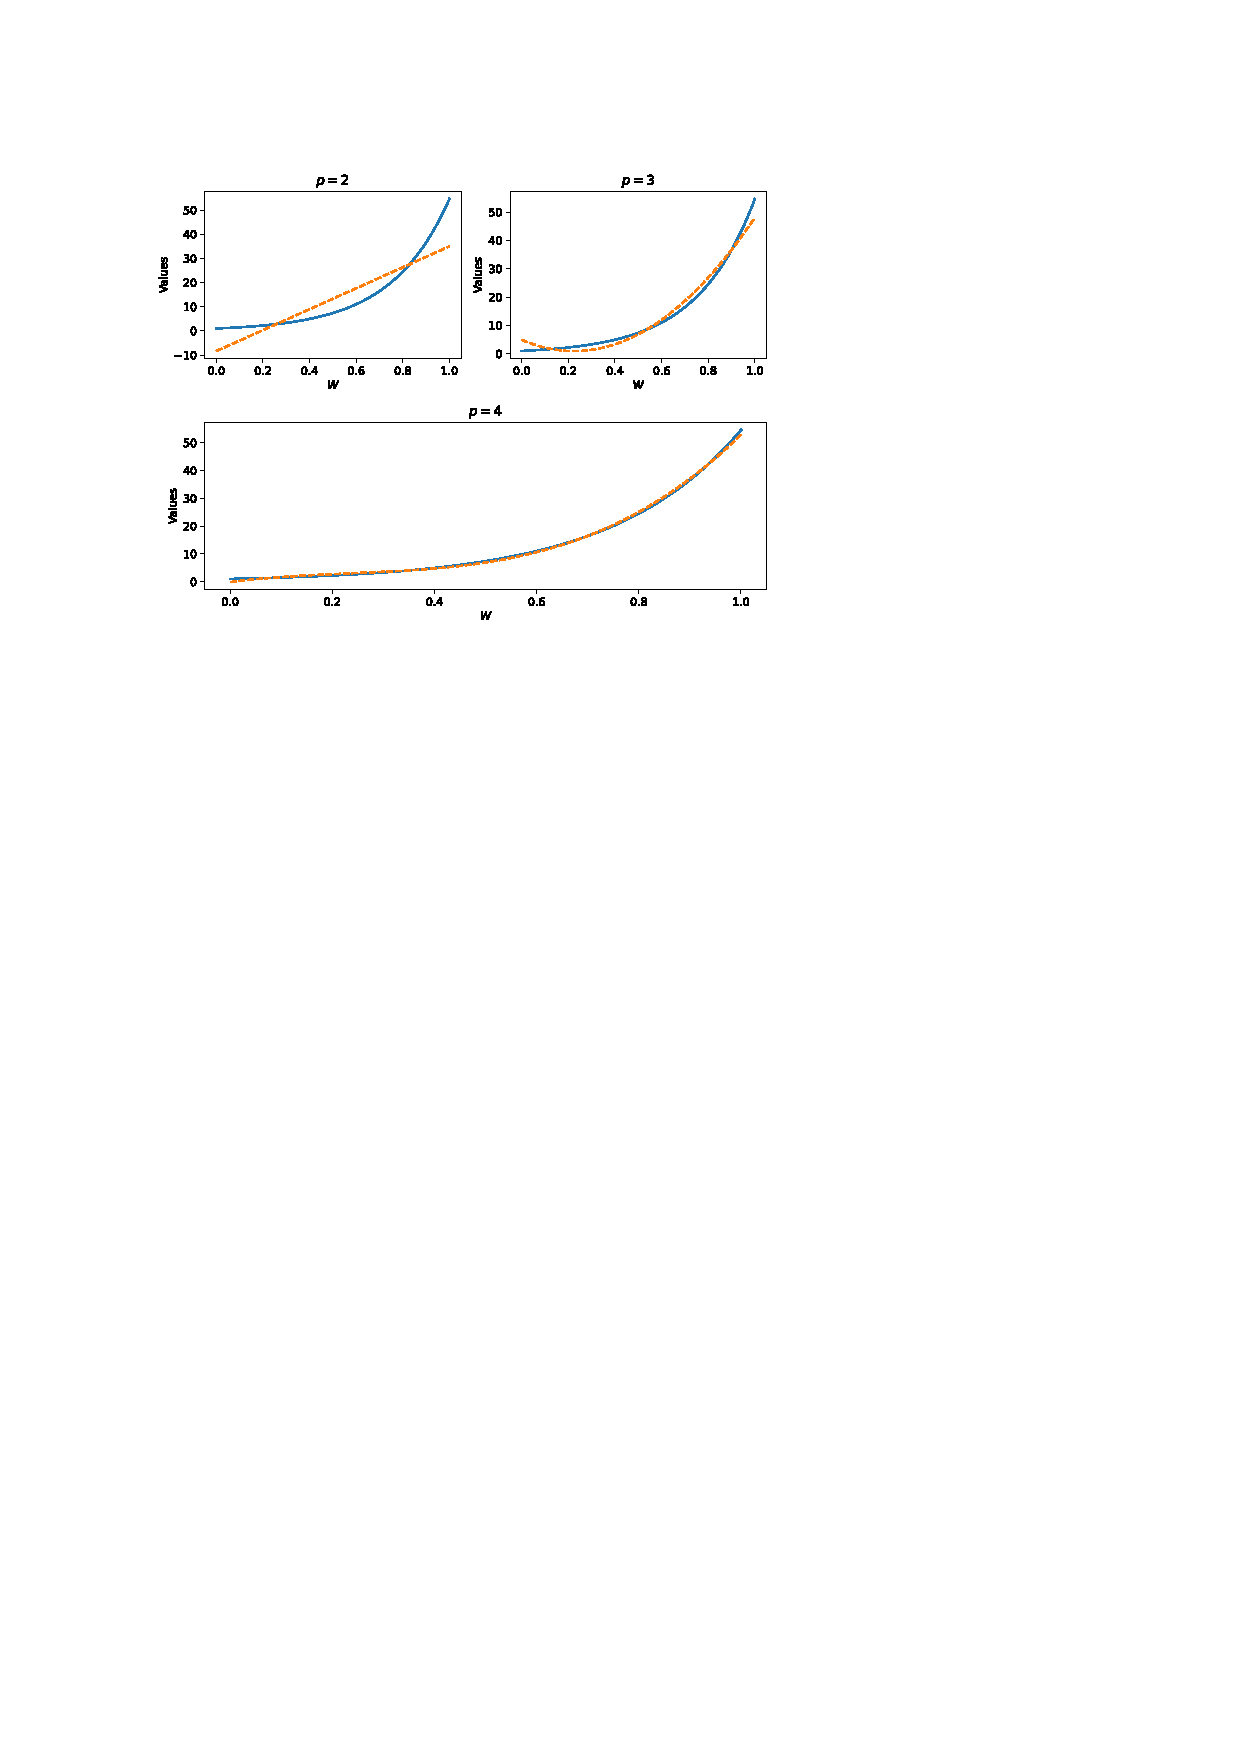
\includegraphics[width=\textwidth]{img/linear_approx.pdf}
        \end{column}
        
    \end{columns}

    
    
\end{frame}





% %%%%%%%%%%%%%%%%%%%%%%%%%%%%%%%%%%%%%%%%%%%%%%%%%%%%%%%%%%%%%%%%%%%%%%%%%%%%%%%%
% \begin{frame}
%     \begin{equation*}
%         g(W) = \EE [Y \vert W]
%     \end{equation*}
%     CEF $g(W)$ solves best prediction problem:
%     \begin{equation*}
%         \min_{m(W)} \EE \left[ \left( Y - m(W) \right)^2\right]
%     \end{equation*} 
% \end{frame}


% %%%%%%%%%%%%%%%%%%%%%%%%%%%%%%%%%%%%%%%%%%%%%%%%%%%%%%%%%%%%%%%%%%%%%%%%%%%%%%%%
% \begin{frame}{Regression of grouped data}

% Use the law of iterated expectations on the regression coefficient $\beta$:
% \begin{align*}
% \beta =& \EE [X_i X_i^\prime]^{-1} \EE [X_i Y_i] \\
% =& \EE \left[ \left. \EE [X_i X_i^\prime]^{-1} \EE [X_i Y_i] \right\vert X_i \right]\\
% =& \EE [X_i X_i^\prime]^{-1} \EE [X_i \EE [Y_i \vert X_i]]
% \end{align*}
% Regression coefficients can be obtained by using $\EE [Y_i \vert X_i]$ as a dependent variable instead of $Y_i$ itself


% \end{frame}

% %%%%%%%%%%%%%%%%%%%%%%%%%%%%%%%%%%%%%%%%%%%%%%%%%%%%%%%%%%%%%%%%%%%%%%%%%%%%%%%%
% \begin{frame}{Regression of grouped data}

% \begin{figure}
% 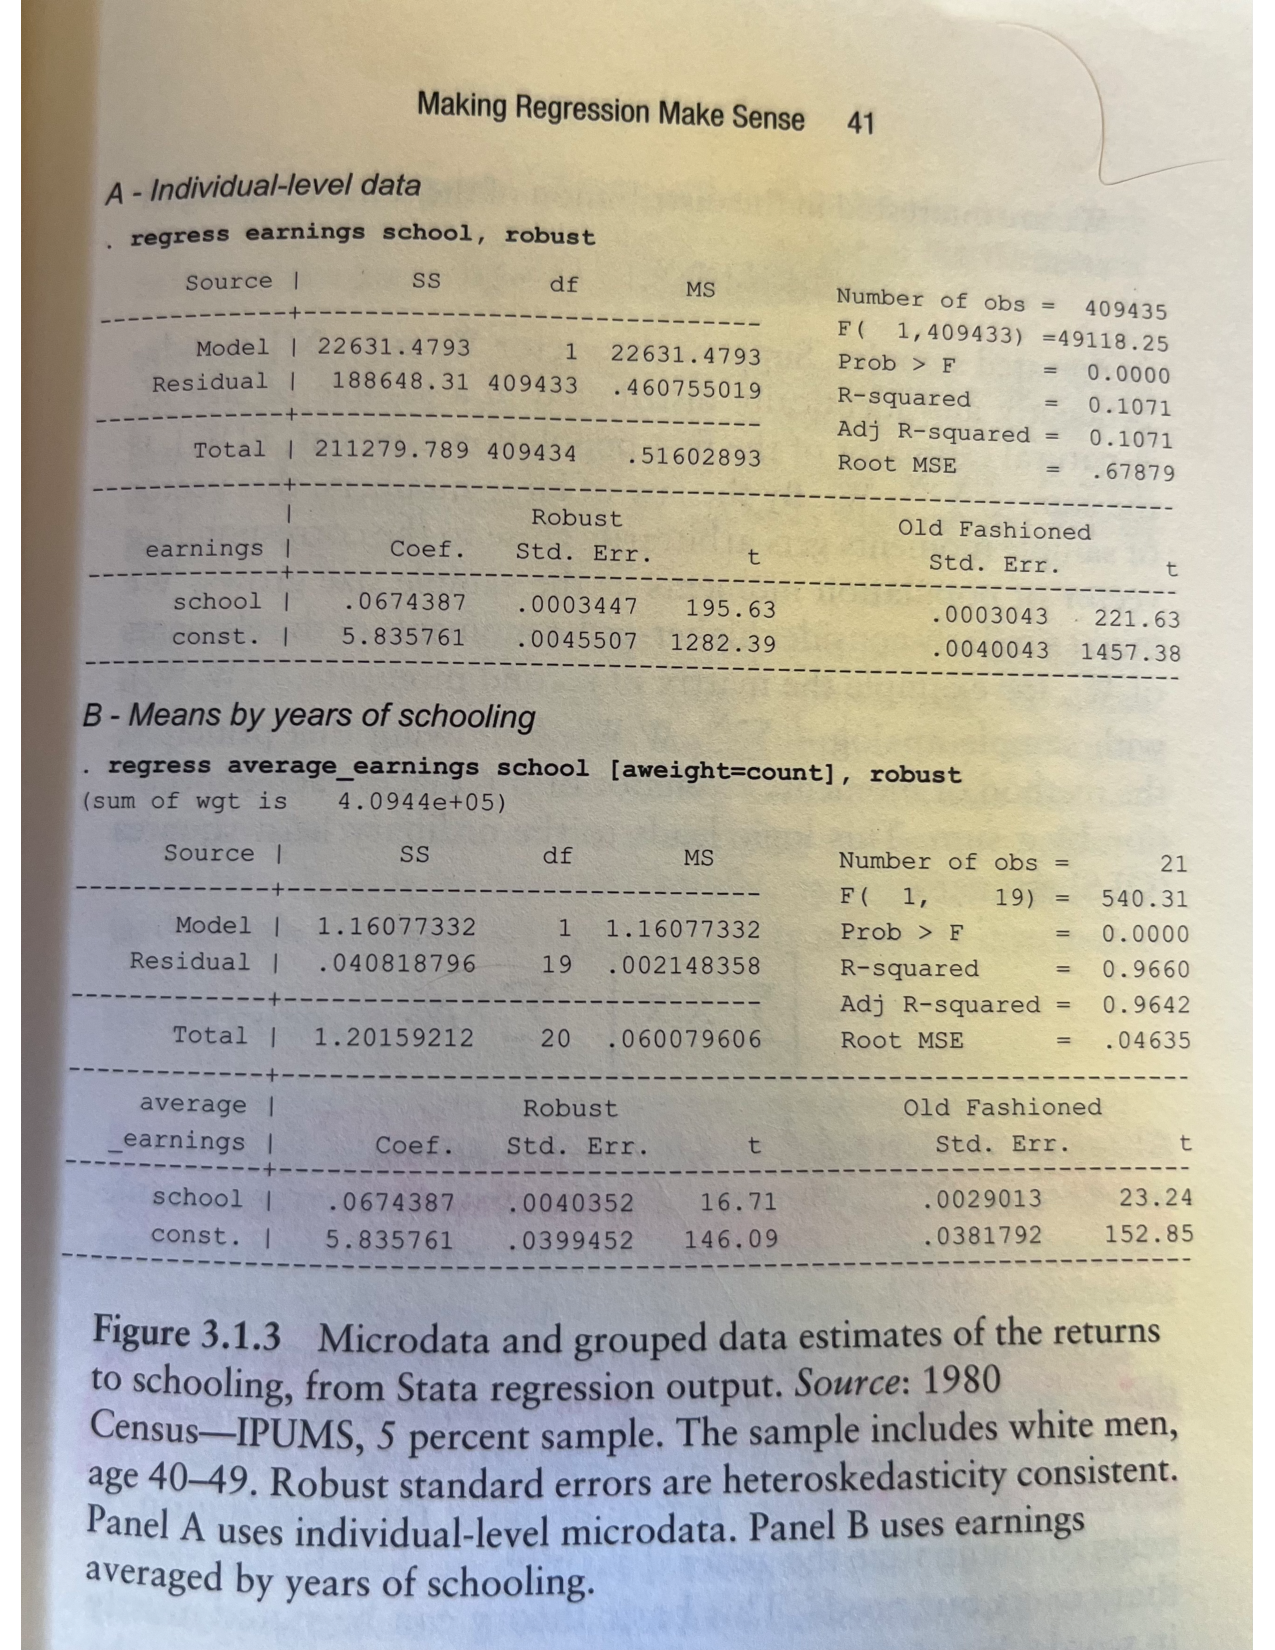
\includegraphics[scale=0.25]{img/fig-3-1-3.pdf}
% \end{figure}

% \end{frame}

%%%%%%%%%%%%%%%%%%%%%%%%%%%%%%%%%%%%%%%%%%%%%%%%%%%%%%%%%%%%%%%%%%%%%%%%%%%%%%%%
\section[Finite]{Statistical properties of least squares}
\miniframesoff
\begin{frame}
    \tableofcontents[currentsection]
\end{frame}
\miniframeson
%%%%%%%%%%%%%%%%%%%%%%%%%%%%%%%%%%%%%%%%%%%%%%%%%%%%%%%%%%%%%%%%%%%%%%%%%%%%%%%%


% %%%%%%%%%%%%%%%%%%%%%%%%%%%%%%%%%%%%%%%%%%%%%%%%%%%%%%%%%%%%%%%%%%%%%%%%%%%%%%%%
\begin{frame}{Statistical properties of least squares}
    In practice, the researcher doesn't have access to the population, but rather a sample:
    \begin{equation*}
        \{ (Y_i, X_i) \}_{i=1}^n = ((Y_1, X_1), (Y_2, X_2), \dots, (Y_n, X_n))
    \end{equation*}

    Assume \textbf{random sample} from $(Y, X)$
    \begin{itemize}
        \item Assume sample is \textbf{independently and identically distributed (iid)}
        \item Independent random draws from a population
    \end{itemize}
\end{frame}

%%%%%%%%%%%%%%%%%%%%%%%%%%%%%%%%%%%%%%%%%%%%%%%%%%%%%%%%%%%%%%%%%%%%%%%%%%%%%%%%
\begin{frame}{BLP problem in sample}
    Best linear predictor for $Y$ using $X$:
    \begin{equation*}
        \sum_{j=1}^p \hat{\beta}_j X_j, \quad \text{ for } \hat{\beta} = (\hat{\beta_1}, \dots, \hat{\beta_p})^\prime
    \end{equation*}
    \quad
    Define $\hat{\beta}$ as the solution to the \textbf{Best Linear Prediction Problem in the Sample}, also known as \textbf{Ordinary Least Squares (OLS)}
    \begin{equation*}
    \min_b \mathbb{E}_n [(Y - b^\prime \XX)^2] = \min_b \underbrace{\frac{1}{n} \sum_{i=1}^n (Y_i - b^\prime \XX_i)^2}_{\text{MSE}}
    \end{equation*}
    \begin{itemize}
        \item Find the $b$ that minimizes the sample MSE
    \end{itemize}
    Sample normal equation:
    \begin{equation*}
        \EE_n [(Y - \hat{\beta}^\prime \XX) \XX]
    \end{equation*}
    Decomposition:
    \begin{align*}
        Y_i = \hat{\beta}^\prime \XX_i + \hat{\epsilon}_i, \quad \mathbb{E}_n [\hat{\epsilon}_i \XX_i] = 0
    \end{align*}
    Where $\epsilon$ are the residuals or in-sample regression errors, $\hat{\epsilon_i} = Y_i - \beta^\prime \XX_i$
\end{frame}

%%%%%%%%%%%%%%%%%%%%%%%%%%%%%%%%%%%%%%%%%%%%%%%%%%%%%%%%%%%%%%%%%%%%%%%%%%%%%%%%
\begin{frame}{Prediction error}
    If best linear prediction rule in the population is $\beta^\prime \XX$, 
    \begin{itemize}
        \item Question: does $\hat{\beta}^\prime \XX$ (from data) approximate $\beta^\prime \XX$ well?
        \item If so, this model gives us the best predictor of $Y$ with future realized values of $\XX$
    \end{itemize}

    \vspace{2ex}
    One problem: Trying to estimate $p$ parameters $\beta = (\beta_1, \dots, \beta_p)^\prime$ 
    \begin{itemize}
        \item Intuitively: $n$ data observations, and $p$ parameters
        \item [$\implies$] want more data than parameters
        \item [$\implies$] want $n/p$ is large or $p/n$ is small
    \end{itemize}
    Define root mean-squared approximation error as:
    \begin{equation*}
        \sqrt{\EE_\XX [(\beta^\prime \XX - \hat{\beta}^\prime \XX)^2]} = 
        \sqrt{(\hat{\beta} - \beta)^\prime \EE_\XX [\XX \XX^\prime] (\hat{\beta} - \beta)}
    \end{equation*}
    \textbf{Want to show:} this prediction error from estimating the best linear predictor is reasonable.

    
\end{frame}

%%%%%%%%%%%%%%%%%%%%%%%%%%%%%%%%%%%%%%%%%%%%%%%%%%%%%%%%%%%%%%%%%%%%%%%%%%%%%%%%
\begin{frame}{Approximation of BLP by OLS}
    RMSE for BLP approximation:
    \begin{equation*}
        \sqrt{\EE_\XX [(\beta^\prime \XX - \hat{\beta}^\prime \XX)^2]} = 
        \sqrt{(\hat{\beta} - \beta)^\prime \EE_\XX [\XX \XX^\prime] (\hat{\beta} - \beta)}
    \end{equation*}

    \textbf{Theorem 1.3.1.: Approximation of BLP by OLS}: Under regularity conditions, the RMSE is bounded by:
    \begin{equation*}
        \text{const}_{p, \alpha} 
        \cdot \underbrace{\sqrt{\EE [\epsilon^2]}}_{\text{noise}}
        \sqrt{p/n}
    \end{equation*}
    where this inequality holds with probability approaching $1 - \alpha$ as $n \to \infty$, and $ \text{const}_{p, \alpha}$ is a constant that depends on the distribution of $(Y, X)$. 
    
    \pause
    \vspace{2ex}    
    \textbf{What does this mean?}
    \begin{itemize}
        \item Under certain conditions, the prediction error from BLP of $Y$ using $X$ scales like the noise level multiplied by $\sqrt{p/n}$
        \item [$\implies$] How small $p/n$ is impacts approximation error
    \end{itemize}

    \vspace{2ex}
    \textbf{Example:} if $p/n$ is small (say, $p/n \approx 0$)
    \begin{equation*}
        \sqrt{\EE_\XX [(\beta^\prime \XX - \hat{\beta}^\prime \XX)^2]} \approx 0
    \end{equation*}
    $\implies$ sample BLP approximates population BLP well. 
    (Source: \href{https://causalml-book.org/chapters/CausalML_chap_1.pdf}{Causal ML book, Chapter 1})

\end{frame}

%%%%%%%%%%%%%%%%%%%%%%%%%%%%%%%%%%%%%%%%%%%%%%%%%%%%%%%%%%%%%%%%%%%%%%%%%%%%%%%%
\begin{frame}{Analysis of variance}
    Analysis of variance involves the decomposition of the variation of $Y$ into explained an unexplained parts. BLP problem's provided decomposition:
    \begin{equation*}
        Y = \beta^\prime \XX + \epsilon, \quad \EE [\epsilon \XX] = 0
    \end{equation*}
    Variation of $Y$ (second moment):
    \begin{align*}
        \EE[Y^2] =& \EE [(\beta^\prime \XX + \epsilon)^2] \\
        % =& \EE [(\beta^\prime \XX)^2 + \beta^\prime \XX \epsilon + \epsilon^2] \\
        =& \EE [(\beta^\prime \XX)^2] + 2 \EE [\beta^\prime \XX \epsilon] + \EE [\epsilon^2] \\
        =& \EE [(\beta^\prime \XX)^2] + 2 \beta^\prime \EE [\XX \epsilon] + \EE [\epsilon^2] \\
        =& \underbrace{\EE [(\beta^\prime \XX)^2 ]}_{\text{explained}} + \underbrace{\EE [\epsilon^2]}_{\text{residual}} 
    \end{align*}
    Decompose variation in $Y$ into \textbf{explained variation} and \textbf{residual variation}.
    \begin{equation*}
        \text{MSE}_{\text{Pop}} = \EE [\epsilon^2]
    \end{equation*}
    Ratio of explained variation to total variation:
    \begin{equation*}
        R^2_{\text{pop}} = \frac{\EE[(\beta^\prime \XX)^2]}{\EE[Y^2]} = 1 - \frac{\EE [\epsilon^2]}{\EE [Y^2]}
    \end{equation*}
    $\implies$ $R^2_{\text{pop}}$ is the proportion of variation of $Y$ explained by the BLP

    % TODO: be able to explain the difference between this and traditional ANOVA (i.e. one is centered, this one is not)
\end{frame}

%%%%%%%%%%%%%%%%%%%%%%%%%%%%%%%%%%%%%%%%%%%%%%%%%%%%%%%%%%%%%%%%%%%%%%%%%%%%%%%%
\begin{frame}{Analysis of variance in sample}
    Analysis of variance involves the decomposition of the variation of $Y$ into explained an unexplained parts. BLP problem's provided decomposition:
    \begin{equation*}
        Y_i = \hat{\beta}^\prime \XX_i + \hat{\epsilon}_i
    \end{equation*}
    Orthogonality condition from normal equation yields decomposition of variation of $Y$ :
    \begin{align*}
        \mathbb{E}_n[Y^2] =& \mathbb{E}_n [(\hat{\beta}^\prime \XX + \hat{\epsilon})^2] \\
        % =& \EE [(\beta^\prime \XX)^2 + \beta^\prime \XX \epsilon + \epsilon^2] \\
        =& \underbrace{\mathbb{E}_n [(\hat{\beta}^\prime \XX)^2 ]}_{\text{explained}} + \underbrace{\mathbb{E}_n [\hat{\epsilon}^2]}_{\text{residual}} 
    \end{align*}
    Decompose variation in $Y$ into \textbf{explained variation} and \textbf{residual variation}.
    \begin{equation*}
        \text{MSE}_{\text{sample}} = \mathbb{E}_n [\hat{\epsilon}^2]
    \end{equation*}
    Ratio of explained variation to total variation:
    \begin{equation*}
        R^2_{\text{sample}} = \frac{\mathbb{E}_n[(\hat{\beta}^\prime \XX)^2]}{\mathbb{E}_n[Y^2]} = 1 - \frac{\mathbb{E}_n [\hat{\epsilon}^2]}{\mathbb{E}_n [Y^2]} \in [0, 1]
    \end{equation*}
    $\implies$ $R^2_{\text{sample}}$ is the proportion of variation of $Y$ explained by the BLP
\end{frame}

%%%%%%%%%%%%%%%%%%%%%%%%%%%%%%%%%%%%%%%%%%%%%%%%%%%%%%%%%%%%%%%%%%%%%%%%%%%%%%%%
\begin{frame}{Analysis of variance in sample and population}
    By law of large numbers, when $p/n$ is small:
    \begin{equation*}
        \mathbb{E}_n [\hat{\epsilon}^2] \approx \EE [\epsilon^2], \quad 
        \mathbb{E}_n[(\hat{\beta}^\prime \XX)^2] \approx \EE[(\beta^\prime \XX)^2], \quad
        \mathbb{E}_n [\hat{\epsilon}^2] \approx \EE [\epsilon^2]
    \end{equation*}

    \begin{itemize}
        \item [$\implies$] When $p/n$ is small and $n$ is large:
    \end{itemize}
    \begin{equation*}
        \text{MSE}_{\text{sample}} \approx \text{MSE}_{\text{Pop}}
        \quad R^2_{\text{sample}} \approx R^2_{\text{pop}} 
    \end{equation*}

    \vspace{2ex} 
    \textbf{Question: } what happens when $p/n$ is not small?
\end{frame}

%%%%%%%%%%%%%%%%%%%%%%%%%%%%%%%%%%%%%%%%%%%%%%%%%%%%%%%%%%%%%%%%%%%%%%%%%%%%%%%%
\begin{frame}{Example: $n = p = 3$}
  Three people with outcomes $Y = (5,\, 2,\, 8)'$, and one dummy per person:
  \[
    \underbrace{\begin{bmatrix} 5 \\ 2 \\ 8 \end{bmatrix}}_{Y}
    =
    \underbrace{\begin{bmatrix}
      1 & 0 & 0 \\
      0 & 1 & 0 \\
      0 & 0 & 1
    \end{bmatrix}}_{X}
    \underbrace{\begin{bmatrix} \hat\beta_1 \\ \hat\beta_2 \\ \hat\beta_3 \end{bmatrix}}_{\hat\beta}
    \quad \Rightarrow \quad
    \hat\beta = \begin{bmatrix} 5 \\ 2 \\ 8 \end{bmatrix}
  \]
  Residuals:
  \[
    \hat\epsilon = Y - X\hat\beta
    = \begin{bmatrix} 5 \\ 2 \\ 8 \end{bmatrix}
    - \begin{bmatrix} 5 \\ 2 \\ 8 \end{bmatrix}
    = \begin{bmatrix} 0 \\ 0 \\ 0 \end{bmatrix}
    \quad \Rightarrow \quad
    \text{MSE}_{sample} = 0,\; R^2_{sample} = 1.
  \]

  \begin{align*}
    \text{MSE}_{sample} &=  \mathbb{E}_n [\hat{\epsilon}^2] = 0 \\
     R^2_{\text{sample}} &= 1 - \frac{\mathbb{E}_n [\hat{\epsilon}^2]}{\mathbb{E}_n [Y^2]} = 1
  \end{align*}

  \begin{itemize}
    \item [$\implies$] This would happen no matter the true value of $\text{MSE}_{\text{pop}}$ and $R^2_{\text{pop} }$
    \item [$\implies$] This is an example of \textbf{overfitting}, when $n=p$
  \end{itemize}
  % TODO: make sure you understand 
\end{frame}

%%%%%%%%%%%%%%%%%%%%%%%%%%%%%%%%%%%%%%%%%%%%%%%%%%%%%%%%%%%%%%%%%%%%%%%%%%%%%%%%
\begin{frame}{Overfitting: computational example}
    Suppose $X \sim N(0, \mathbb{I}_p)$ and $Y \sim N(0, 1)$ are statistically independent. It follows that the best linear predictor of $Y$ is $\beta^\prime X = 0$ (i.e. $\beta = 0$). $R^2_{\text{pop}}$, the proportion of variation of $Y$ explained by the BLP, is 0 ($R^2_{\text{pop}} = 0$).

    \begin{itemize}
        \item If $p=n$, then the typical $R^2_{\text{sample}}$ is $\approx 1$
        \item If $p = n/2$, then the typical $R^2_{\text{sample}}$ is $\approx 0.5$
        \item If $p = n/20$, then the typical $R^2_{\text{sample}}$ is $\approx 0.05$
    \end{itemize}

\end{frame}

%%%%%%%%%%%%%%%%%%%%%%%%%%%%%%%%%%%%%%%%%%%%%%%%%%%%%%%%%%%%%%%%%%%%%%%%%%%%%%%%
\begin{frame}{Adjusted $R^2$ and $MSE$}
Provided $p < n$, better measures of out-of-sample predictive
ability are the "adjusted" $R^2$ and MSE:
\begin{align*}
    MSE_{\text{adjusted}} = \frac{n}{n - p} \mathbb{E}_n[\hat{\epsilon}^2], \quad R^2_{\text{adjusted}} = 1 - \frac{n}{n - p} \frac{\mathbb{E}_n[\hat{\epsilon}^2]}{\mathbb{E}_n [Y^2]}
\end{align*}

\begin{itemize}
    \item Models with many parameters $p$ may exhibit overfitting
    \item Number of parameters incorporated in an attempt to
account for this phenomenon
\end{itemize}

% TODO: adjusted R^2 is a sample only phenomenom, correct?

\end{frame}

%%%%%%%%%%%%%%%%%%%%%%%%%%%%%%%%%%%%%%%%%%%%%%%%%%%%%%%%%%%%%%%%%%%%%%%%%%%%%%%%
\begin{frame}{Sample splitting}

    How should we measure the predictive ability of the linear model (or other nonlinear model) more reliably, even when $p/n$ is not small?

    \vspace{2ex}
    \begin{itemize}
        \item [$\implies$] A general way to measure predictive performance is to perform \textbf{data splitting}
    \end{itemize}

\begin{enumerate}
    \item Split data randomly into \textbf{training} and \textbf{test} sets

    \item Using the \textbf{training sample}, for estimating (train) the prediction rule.

    \item Using the \textbf{testing sample}, evaluate the quality of the prediction rule, recording out-of-sample MSE and $R^2$
\end{enumerate}

\vspace{2ex}
\emph{Without sample splitting:} predictive model is trained on a sample and the real test of its predictive ability happens when ``new, unseen'' observations arrive

\vspace{2ex}
\emph{With sample splitting: } preserve an ``unseen'' set of observations on which to test our model, mimicking this process of ex-post performance assessment

% TODO: cite Athey paper on ML in econ/sample splitting?

\end{frame}


%%%%%%%%%%%%%%%%%%%%%%%%%%%%%%%%%%%%%%%%%%%%%%%%%%%%%%%%%%%%%%%%%%%%%%%%%%%%%%%%
\begin{frame}{ML vs econometrics}

    Differences between machine learning (statistical) methods and econometrics:
    \begin{itemize}
        \item ML more concerned with overfitting; sample splitting is a straightforward way of addressing that
        \item ML less concerned than econometrics with formal results that particular methods are superior in large samples (i.e. asymptotic results)
    \end{itemize}
    Over the past 10 years, econometrics and ML have begun to borrow heavily from one another in causal inference.

    \vspace{2ex}
    %TODO: describe Susan AThey paper

\end{frame}


%%%%%%%%%%%%%%%%%%%%%%%%%%%%%%%%%%%%%%%%%%%%%%%%%%%%%%%%%%%%%%%%%%%%%%%%%%%%%%%%
\section[Inference]{Predictive Effects}
\miniframesoff
\begin{frame}
    \tableofcontents[currentsection]
\end{frame}
\miniframeson
%%%%%%%%%%%%%%%%%%%%%%%%%%%%%%%%%%%%%%%%%%%%%%%%%%%%%%%%%%%%%%%%%%%%%%%%%%%%%%%%

%%%%%%%%%%%%%%%%%%%%%%%%%%%%%%%%%%%%%%%%%%%%%%%%%%%%%%%%%%%%%%%%%%%%%%%%%%%%%%%%
\begin{frame}{Predictive Effect}
    
    Partition the regressors $X$ into:
    \begin{equation*}
        X = (D, W)^\prime
    \end{equation*}
    \begin{itemize}
        \item $D$: target regressor of interest
        \item $W$: other regressors (controls)
    \end{itemize}
    Can write:
    \begin{equation*}
        Y = \underbrace{\beta_1 D + \beta_2^\prime W}_{\text{predicted value}} + \epsilon
    \end{equation*}
    \textbf{Key question:}  How does the predicted value of $Y$ change if $D$ increases by a unit while $W$ remains unchanged?

    \vspace{2ex} \textbf{Example:} What is the difference in predicted wages between female and non-female workers with the same job-relevant characteristics
    \begin{itemize}
        \item $D$: female indicator
        \item $W$: experience, educational, occupational, and geographic characteristics
        \item Coefficient of interest: $\beta_1$
    \end{itemize}

\end{frame}

%%%%%%%%%%%%%%%%%%%%%%%%%%%%%%%%%%%%%%%%%%%%%%%%%%%%%%%%%%%%%%%%%%%%%%%%%%%%%%%%
\begin{frame}{Partialing out operation}
    For some random variable $V$, created a residualized variable $\tilde{V}$ by subtracting the part of $V$ linearly predicted by $W$
    \begin{equation*}
        \tilde{V} = V - \gamma_{VW}^\prime W, \quad \gamma_{VW} = \arg \min_{\gamma} \EE [(V - \gamma^\prime W)^2]
    \end{equation*}
    If $V$ is a vector, applying the operation to each component:
    \begin{equation*}
        {\color{MainBlue}Y = \nu V + \mu U} \implies \tilde{Y} = \nu \tilde{V} + \mu \tilde{U}
    \end{equation*}

    \vspace{1ex}
    \textbf{Why does this matter?}
    \begin{itemize}
        \item Can ``partial out'' predictive power of $W$
        \item Becomes very important in dimensionality reduction - when $p/n$ is not small
    \end{itemize}

\end{frame}

%%%%%%%%%%%%%%%%%%%%%%%%%%%%%%%%%%%%%%%%%%%%%%%%%%%%%%%%%%%%%%%%%%%%%%%%%%%%%%%%
\begin{frame}{Partialing out operation proof}
    Want to show: ${Y = \nu V + \mu U} \implies \tilde{Y} = \nu \tilde{V} + \mu \tilde{U}$, where:
    \begin{equation*}
        \tilde{V} = V - \gamma_{VW}^\prime W, \quad \gamma_{VW} = \arg \min_{\gamma} \EE [(V - \gamma^\prime W)^2]
    \end{equation*}
        \textbf{Proof:} $\gamma_{VW}$ is the BLP of $V$ given $W$ $\implies$ $\tilde{V}$ is a residual $\implies$ normal equation:
    \begin{align*}
        % \gamma_{VW} =& \arg \min_{\gamma} \EE [(V - \gamma^\prime W)^2] \\
        % \tilde{V} =&  \underbrace{V - \gamma_{VW} W}_{\text{residual of linear prediction}} \\
        \EE [\tilde{V} W] = 0
    \end{align*}
    We will define $\gamma^* = \nu \gamma_{VW} + \mu \gamma_{UW}$ as a candidate BLP of $Y$ given $W$:
    \begin{align*}
        \nu \tilde{V} + \mu \tilde{U} =& \nu( V - \gamma_{VW}^\prime W) + \mu ( U - \gamma_{UW}^\prime W) \\
        % =& \nu V - \nu \gamma_{VW}^\prime W + \mu U - \mu \gamma_{UW}^\prime W \\
        =& \underbrace{\color{MainBlue}\nu V + \mu U}_{\text{Def of $Y$}} - \underbrace{(\nu \gamma_{VW} + \mu \gamma_{UW})^\prime W}_{\text{Linear function of $W$}} \\
        =& {\color{MainBlue}Y} - {\gamma^*}^\prime W
    \end{align*}
    $\gamma^*$ is the BLP of $Y$ if normal equation holds. \textbf{Check orthogonality.}
    \begin{equation*}
        \EE\big[W(\nu \tilde{V} + \mu \tilde{U})\big]
        = \nu \underbrace{\EE[W \tilde{V}]}_{=0} + \mu \underbrace{\EE[W \tilde{U}]}_{=0} = 0 .
    \end{equation*}
    So $\gamma^*$ solves the normal equations for $Y$, i.e.\ $\gamma^*$ is a valid $\gamma_{YW}$, and
    \begin{equation*}
        \tilde{Y} = Y - {\gamma^*}' W = \nu \tilde{V} + \mu \tilde{U}. 
    \end{equation*}

\end{frame}


%%%%%%%%%%%%%%%%%%%%%%%%%%%%%%%%%%%%%%%%%%%%%%%%%%%%%%%%%%%%%%%%%%%%%%%%%%%%%%%%
\begin{frame}{Partialing out regression equation}
    Regression Equation:
    \begin{equation*}
        Y = \beta_1 D + \beta_2^\prime W + \epsilon \implies \tilde{Y} = \beta_1 \tilde{D} + \beta_2^\prime \tilde{W} + \epsilon
    \end{equation*}
    Partial out $W$:
    \begin{equation*}
        \tilde{Y} = \beta_1 \tilde{D} + \beta_2 \tilde{W} + \tilde{\epsilon}
    \end{equation*}
    which simplifies to:
    \begin{equation*}
        \tilde{Y} = \beta_1 \tilde{D} + \epsilon, \quad \EE [\epsilon \tilde{D}] = 0
    \end{equation*}
    \begin{itemize}
        \item $\tilde{W} = 0$ because BLP of $W$ given $W$ is just $W$
        \item $\epsilon$ unchanged because $\epsilon$ is linearly unpredictable by $X$ $\implies$ $\epsilon$ is linearly unpredictable by $W$ $\implies$ $\tilde{\epsilon} = \epsilon$  
    \end{itemize}

    \vspace{2ex}
    Because $\tilde{D}$ is a linear function of $X = (D, W^\prime)^\prime$, and $\epsilon$ is orthogonal to $X$, $\EE[\epsilon \tilde{D}] = 0$
    \begin{itemize}
        \item This is the normal equation for the population regression of $\tilde{Y}$ on $\tilde{D}$
    \end{itemize}

\end{frame}


%%%%%%%%%%%%%%%%%%%%%%%%%%%%%%%%%%%%%%%%%%%%%%%%%%%%%%%%%%%%%%%%%%%%%%%%%%%%%%%%
\begin{frame}{Frisch-Waugh-Lovell}

    Assume:
    \begin{itemize}
        \item $Y$, $D$, $W$ have finite second moments
        \item $D$ is not perfectly predictable by $W$ $\implies$ $\EE[\tilde{D}^2] > 0$
    \end{itemize} 
    \vspace{2ex}
    Then population linear regression coefficient $\beta_1$ can be recovered from population regression of $\tilde{Y}$ on $\tilde{D}$:
    \begin{equation*}
        \beta_1 = \arg \min_{b_1} \EE [(\tilde{Y} - b_1 \tilde{D})^2] = (\EE [\tilde{D}^2])^{-1} \EE [\tilde{D} \tilde{Y}]
    \end{equation*}
\end{frame}

%%%%%%%%%%%%%%%%%%%%%%%%%%%%%%%%%%%%%%%%%%%%%%%%%%%%%%%%%%%%%%%%%%%%%%%%%%%%%%%%
\begin{frame}{Partialing out in sample}
    Let $\check{V}_i$ be the residual left after predicting $V_i$ with controls $W_i$ in the sample. 
    \begin{equation*}
        \check{V}_i = V_i - \hat{\gamma}_{VW}^\prime W_i, \quad \hat{\gamma}_{VW} = \arg \min_{\gamma} \mathbb{E}_n [(V - \gamma^\prime W)^2]
    \end{equation*}
    Assume $\mathbb{E}_n \left[ \check{D}^2 \right] > 0$.

    \vspace{2ex}
    Apply Frisch-Waugh-Lovell to the sample:
    \begin{equation*}
        \hat{\beta}_1 = \arg \min_{b} \mathbb{E}_n \left[ \left( \check{Y} - b \check{D} \right)^2 \right]
        = \left( \mathbb{E}_n \left[ \check{D}^2 \right] \right)^{-1} \mathbb{E}_n \left[ \check{D} \check{Y} \right],
    \end{equation*}
    \begin{itemize}
        \item [$\implies$] Sample linear regression of $Y$ on $D$ and $W$ gives the same $\hat{\beta}_1$ as estimator obtained via partialing out
    \end{itemize}

    \vspace{2ex}
    \textbf{Note of first step} (partialing out regression):
    \begin{itemize}
        \item Need to estimate residuals $\check{V}_i$
        \item If $p/n$ is small, sample linear regression produces good estimates of the residuals
        \item If $p/n$ NOT small, sample linear regression for partialling out may not produce good estimates of residuals
        \item [$\implies$] Need to use strategy that reduces dimensionality (like LASSO)
    \end{itemize}

\end{frame}

%%%%%%%%%%%%%%%%%%%%%%%%%%%%%%%%%%%%%%%%%%%%%%%%%%%%%%%%%%%%%%%%%%%%%%%%%%%%%%%%
\begin{frame}{Adaptive statistical inference}
    \textbf{Question: } if $\check{Y}$ and $\check{D}$ are computed using $W$, does first-tage estimation effect distribution of $\hat{\beta}_1$?
    \begin{itemize}
        \item [$\implies$] Under regularity conditions and $p/n \approx 0$, the estimation error in $\check{D}$ and $\check{Y}$ has no first order effect on the stochastic behavior of $\hat{\beta}_1$:
    \end{itemize}
    \begin{equation*}
        \sqrt{n}(\hat\beta_1 - \beta_1) \approx
        \frac{\sqrt{n}\, \mathbb{E}_n[\tilde{D}\epsilon]}{\mathbb{E}_n[\tilde{D}^2]}
        \quad \Rightarrow \quad
        \sqrt{n}(\hat\beta_1 - \beta_1) \overset{a}{\sim} N(0, V),
    \end{equation*}
    \begin{equation*}
        V = \big(\EE[\tilde{D}^2]\big)^{-1} \EE[\tilde{D}^2 \epsilon^2] \big(\EE[\tilde{D}^2]\big)^{-1}.
    \end{equation*}
    Equivalently: $\hat\beta_1 \overset{a}{\sim} N(\beta_1, V/n)$.
    \begin{itemize}
        \item $\hat{\beta}_1$ is approximately normally distributed with mean $\beta_1$ and variance $V/n$.
        \item [$\implies$] $\hat{\beta}_1$ concentrates in a $V/n$-neighborhood of $\beta_1$, with deviations constrained by the normal law
    \end{itemize}
\end{frame}

%%%%%%%%%%%%%%%%%%%%%%%%%%%%%%%%%%%%%%%%%%%%%%%%%%%%%%%%%%%%%%%%%%%%%%%%%%%%%%%%
\begin{frame}{Why ``adaptive''?}
    \begin{itemize}
        \item Estimation of residual $\check{D}$ has a negligible impact on large sample behavior of OLS
        \item Approximation behavior is the same as if we had used true residuals $\tilde{D}$
        % \item The approximation uses the \emph{true} residuals $\tilde{D}$:
            %   estimating them has no \emph{first-order} effect on $\hat\beta_1$.
        \item $\hat\beta_1$ behaves as if we had known $\tilde{Y}, \tilde{D}$ all along.
        \item The estimator minus the estimand is approximately a centered average
              $\Rightarrow$ normality follows from the CLT.
        \item This is a special case of \textbf{Neyman orthogonality}
            
    \end{itemize}
\end{frame}

%%%%%%%%%%%%%%%%%%%%%%%%%%%%%%%%%%%%%%%%%%%%%%%%%%%%%%%%%%%%%%%%%%%%%%%%%%%%%%%%
\begin{frame}{Standard errors and confidence intervals}
    \textbf{Eicker--Huber--White (robust) variance estimator:}
    \begin{equation*}
        \hat{V} = \big(\mathbb{E}_n[\check{D}^2]\big)^{-1}
                  \mathbb{E}_n[\check{D}^2 \hat\epsilon^2]
                  \big(\mathbb{E}_n[\check{D}^2]\big)^{-1},
        \qquad \text{s.e.}(\hat\beta_1) = \sqrt{\hat{V}/n}.
    \end{equation*}
    Valid when $p/n \approx 0$; fails when $p/n$ is not small.
    \medskip

    \textbf{$(1-a)\times 100\%$ confidence interval:}
    \begin{equation*}
        \Big[\hat\beta_1 \pm z_{1-a/2} \sqrt{\hat{V}/n}\Big],
        \qquad \text{e.g. } 95\%: \; \hat\beta_1 \pm 1.96 \sqrt{\hat{V}/n}
    \end{equation*}
    Contains $\beta_1$ approximately $(1-a)\times 100\%$ of the time.
    \medskip

    \footnotesize Avoid the ``classical'' $\frac{n}{n-p}(\mathbb{E}_n[\check{D}^2])^{-1}\mathbb{E}_n[\hat\epsilon^2]$:
    not robust to heteroscedasticity.
\end{frame}
%%%%%%%%%%%%%%%%%%%%%%%%%%%%%%%%%%%%%%%%%%%%%%%%%%%%%%%%%%%%%%%%%%%%%%%%%%%%%%%%
\begin{frame}{Example: wage gap}

    Important question in labor economics: what determines the wage of workers
    \begin{itemize}
        \item Causal question
        \item Today, focus on question from predictive perspective
    \end{itemize}

    \vspace{2ex}
    \emph{Question}:
    \begin{itemize}
        \item How can we use job-relevant characteristics to best predict wages?
        \item Are the difference in predicted wages different for male and female workers with similar job-relevant characteristics
    \end{itemize}

    \vspace{2ex}
    Estimate a linear predictive regression model for log hourly wages using job-relevant characteristics $X$:
    \begin{equation*}
        Y = \beta^\prime X + \epsilon, \quad \epsilon \perp X
    \end{equation*}
    Assess the quality of the prediction rule using out of sample performance
    \begin{itemize}
        \item Question: is there a gap between male and female workers? Does that reflect discrimination?
    \end{itemize}
\end{frame}

\end{document}





